\documentclass[9pt,technote]{IEEEtran}

\usepackage[T1]{fontenc}
\usepackage[utf8]{inputenc}
\usepackage{cite}
\usepackage{newtxtext,newtxmath}
\usepackage{tablefootnote}
\usepackage{graphicx}
\title{Neural Network}
\author{
	Gian Marco Balia\\
	Robotic Engineering - University of Genoa\\
	s4398275@studenti.unige.it
}

\begin{document}

\maketitle

\begin{abstract}
Artificial neural networks are a fundamental approach in machine learning due to their efficiency to model complex relationships and learn meaningful representations from data. Auto-encoders, a specific class of neural networks, are widely used for dimensionality reduction, data compression, and unsupervised learning tasks. This report explores the fundamental principles of neural networks and auto-encoders, analysing their architecture, training process, and practical applications.
\end{abstract}
\begin{IEEEkeywords}
Artificial neural networks, auto-encoder
\end{IEEEkeywords}

\section{Introduction}
Artificial neural networks in the field of machine learning represent an innovative approach to tackling complex problems across various domains, from image processing to sequential data prediction. Auto-encoders are among the earliest neural network architectures designed to learn latent representations of data with an unsupervised approach. They operate by compressing data into a reduced-dimensional space and reconstructing the original input, aiming to capture relevant features and redundancies. \\
The importance of auto-encoders lies in their versatility: they have been successfully applied in tasks such as dimensionality reduction (Hinton e Salakhutdinov, 2006), anomaly detection (Chalapathy e Chawla, 2019), and deep network pre-training. Furthermore, recent advancements, such as the introduction of variational auto-encoders (Kingma e Welling, 2013), have expanded their applications to include synthetic data generation and probabilistic learning. This report aims to provide an analysis of the fundamental concepts related to neural networks and auto-encoders, illustrating practical examples and experiments that demonstrate their effectiveness in real-world applications.
\section{Material and methods}

\subsection{Data processing}
For this analysis, the MNIST dataset (Modified National Institute of Standards and Technology) was used, one of the most well-known datasets for image classification tasks. This dataset contains images of handwritten digits ($0$ to $9$), where each image is gray-scale, has dimensions of $28\times28$ pixels, and each pixel has a value between $0$ and $255$, representing the intensity of the color ($0$ means black, $255$ means white).

After loading the data, it was filtered to include only the digits $1$ and $8$. This reduced the dataset to two classes of interest. The filtered data were then split into distinct datasets: 
\begin{itemize}
	\item \textit{($x_{train}$,$y_{train}$)}:  $80\%$ of the filtered data and contains the training images. It represent as $28\times28$ matrices that describe the pixel values, and the corresponding training labels ($1$ and $8$), which represent the digits associated with the images.
	\item \textit{($x_{train}$,$y_{train}$)}: $20\%$ of the filtered data contains the images for the test. It represent as $28\times28$ matrices that describe the pixel values, and the corresponding labels for the test ($1$ and $8$), which represent the digits associated with the images.
\end{itemize}
Then, the following steps were done to make the data compatible with the model architecture.
\begin{itemize}
	\item \textit{Data Normalization}: to improve performance and ensure compatibility with the model architecture, the data were normalized, converting the pixel values from their original range ($0$-$255$) to a range between $0$ and $1$. This transformation is essential to accelerate convergence during training and reduce the risk of numerical instability.
	\item \textit{Data Reshaping}: since the MNIST images, when loaded, have the shape like a three-dimensional array (\textit{$num_{}samples$}, $28$, $28$), where: \textit{$num_{}samples$} is the number of images in the dataset, and $28x28$ are the dimensions of each image.
	Many deep learning models, require the data to be represented in a four-dimensional format: (\textit{$num_{}samples$}, \textit{height}, \textit{width}, \textit{channels}). In the case of MNIST images, the channels value is $1$ because the images are greyscale.
	Thus, the data were reshaped from the form (\textit{$num_{}samples$}, $28$, $28$) to (\textit{$num_{}samples$}, $28$, $28$, $1$) using the \textit{reshape} command. This step explicitly adds the required depth channel, making the data compatible with the auto-encoder architecture.
\end{itemize}

\subsection{Auto-encoder}
The autoencoder is an artificial neural network model designed to learn a compact and meaningful representation of input data. The model consists of two main parts: the encoder, which receives the input data and compresses it into a lower-dimensional representation, and the decoder, which receives the compressed representation and reconstructs it into the original output data.

The autoencoder model used in this work is composed of the following parts:
\begin{itemize}
	\item \textit{Encoder}: the neural network that receives the input data and compresses it into a lower-dimensional representation. The encoder consists of a series of neural network layers, each applying a nonlinear transformation to the input data.
	\item \textit{Decoder}: the neural network that receives the compressed representation and reconstructs it into the original output data. The decoder consists of a series of neural network layers, each applying a nonlinear transformation to the input data.
	\item \textit{Autoencoder}: the complete model that combines the encoder and decoder. The autoencoder is trained to minimize the reconstruction error, which is the difference between the original input data and the reconstructed output data.
\end{itemize}

The autoencoder model operates as follows: the input data is fed to the encoder, which compresses the data into a lower-dimensional representation. The decoder receives this compressed representation and reconstructs it into the original output data. The reconstruction error is calculated as the difference between the original input data and the reconstructed output data. Finally, the model is trained to minimize the reconstruction error using an the Adam optimizer algorithm (short for “Adaptive Moment Estimation”) to minimize the loss function during the training of neural networks.

\subsection{Model evaluation}
The methods for evaluating the correct implementation of the autoencoder model are different.
The most intuitive method is visual inspection: it involves checking whether the digital reconstruction accurately reflects the original input data (see Fig. \ref{fig:digitalrecostruction})
\begin{figure}
	\centering
	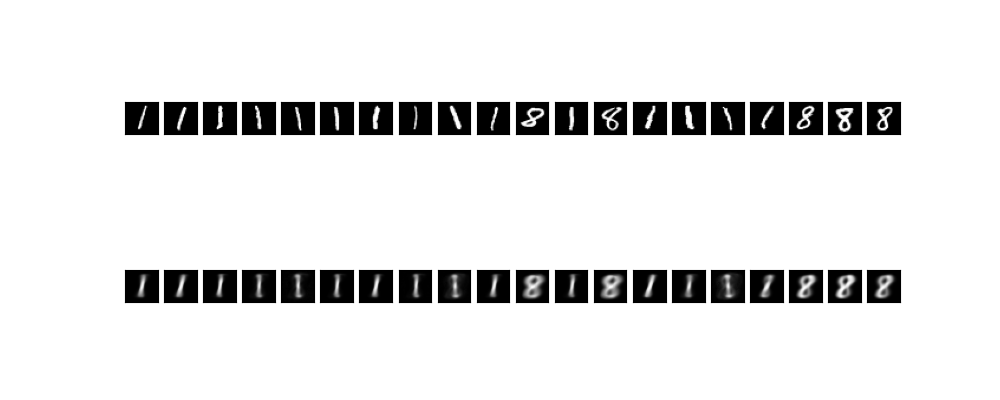
\includegraphics[width=0.7\linewidth]{Resources/DigitalRecostruction}
	\caption{Reconstruction of the digits data $1$ and $8$. In the first row there are the original data digit and in the second row the reconstructed data}
	\label{fig:digitalrecostruction}
\end{figure}

An alternative approach is the use of the VAF (Variance Accounted For), a specific metric for assessing the performance of autoencoders. The VAF indicates the quality of the data reconstruction by evaluating how representative and useful the compressed data is for reconstructing the original input. The VAF is computed as:
\begin{equation*}
<<<<<<< HEAD
<<<<<<< HEAD
	VAF = 1 - \Big(\frac{var(\text{x}_{test} - \text{x}_{pred})}{var(\text{x}_{test})}\Big) \cdot 100
=======
	VAF = 1 - (\frac{variance(\textit{true data} - \textit{predicted data})}{variance(\textit{true data})}) \cdot 100
>>>>>>> 9c67fc0a693e3f5d6bc2b8a22d24ff17f8ab5892
=======
	VAF = 1 - (\frac{variance(\textit{true data} - \textit{predicted data})}{variance(\textit{true data})}) \cdot 100
>>>>>>> 9c67fc0a693e3f5d6bc2b8a22d24ff17f8ab5892
\end{equation*}
where:
$\text{x}_{test}$ represents the original values;
$\text{x}_{pred}$ represents the values reconstructed by the autoencoder.
The calculated values for each reconstructed data point are reported in Fig. \ref{fig:varianceaccountedfor}.
\begin{figure}
	\centering
	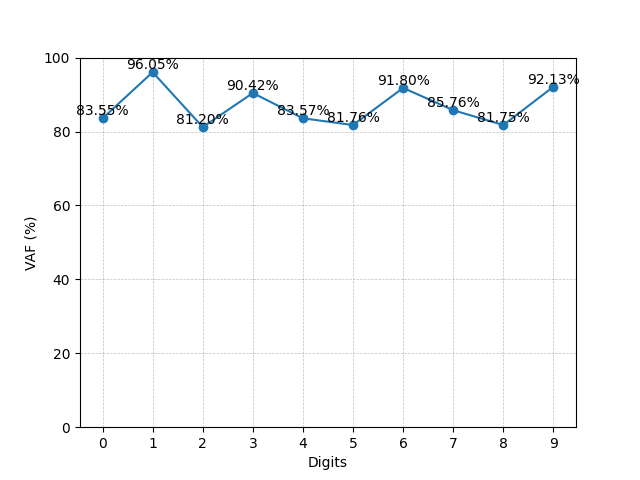
\includegraphics[width=0.7\linewidth]{Resources/VarianceAccountedFor}
	\caption{The figure represented the VAF computed for the digits values $1$ and $8$}
	\label{fig:varianceaccountedfor}
\end{figure}

Finally, another useful method for evaluating the model's implementation is to compute the information loss during reconstruction. This aspect is graphically represented in Fig. \ref{fig:autoencodermodelloss}.
\begin{figure}
	\centering
	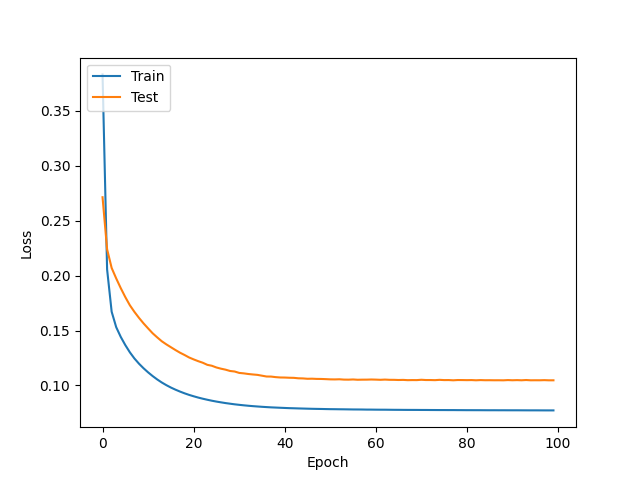
\includegraphics[width=0.7\linewidth]{Resources/AutoencoderModelLoss}
	\caption{The figure represented the information lost during the process}
	\label{fig:autoencodermodelloss}
\end{figure}

\section{Results and Conclusion}
The proper functioning of the autoencoder is demonstrated in Fig. \ref{fig:digitalrecostruction}, which highlights the model's ability to reconstruct the original data with high fidelity. This result showcases the effectiveness of the architecture and the training process in capturing the essential features of the input data while minimizing reconstruction error.

Additionally, Fig. \ref{fig:autoencodermodelloss} illustrates the progressive reduction in information loss as the number of epochs increases, highlighting the steady improvement in model performance. This behavior reflects the optimization of the autoencoder's weights and biases over time, allowing for better alignment between the encoded latent representation and the original data structure.

An analysis of the Variance Accounted For (VAF) values, shown in Fig. \ref{fig:varianceaccountedfor}, provides further insights into the autoencoder's performance across different digital values. For the digital value 1, the VAF reaches 67.85$\%$, indicating the model's strong ability to capture and reconstruct this value with minimal information loss. Conversely, for the digital value 8, the VAF is 49.30$\%$, reflecting greater difficulty in preserving information during reconstruction. These results emphasize the superior performance of the autoencoder with certain values compared to others, likely due to the complexity or distribution of the data associated with each value.

Furthermore, the scatter plot in Fig. \ref{fig:endodeddimentions} represents the latent space encoded by the autoencoder, showing the first two dimensions of the encoded representation. The points are color-coded based on the digital values $1$ (blue) and $8$ (green). This visualization highlights the distinct separation of the two labels in the encoded space, demonstrating the autoencoder's ability to learn meaningful representations.

The cluster corresponding to Label $1$ appears well-defined and compact, suggesting that the autoencoder effectively captures the structure of this value. In contrast, the points associated with Label $8$ exhibit a wider dispersion, reflecting greater variability in the encoded representation. This aligns with the previously observed lower VAF value for Label $8$, indicating that the reconstruction process struggles more with this class.

These differences in the encoded space emphasize the variability in the autoencoder's performance depending on the complexity and distribution of the input data. Future improvements could include enhancing the encoder's ability to capture finer details for more challenging labels, potentially through increased latent dimensionality or advanced regularization techniques.
\begin{figure}
	\centering
	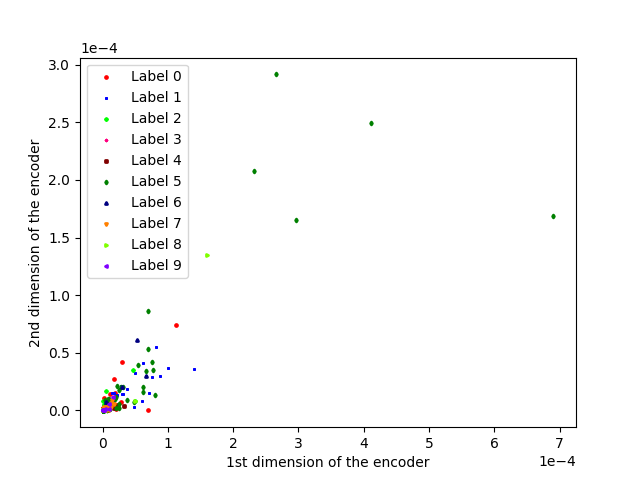
\includegraphics[width=0.7\linewidth]{Resources/EndodedDImentions}
	\caption{Visualization of the latent space encoded by the autoencoder, showing the first two dimensions of the encoded representation. Points are color-coded based on digital values: Label 1 (blue) and Label 8 (green).}
	\label{fig:endodeddimentions}
\end{figure}

%% inserire parte mancante task 0 e aggiungi reference

\end{document}